\documentclass[a4paper,1pt]{jsarticle}


% 数式
\usepackage{amsmath,amsfonts}
\usepackage{bm}
% 画像
\usepackage[dvipdfmx]{graphicx}
\usepackage[dvipdfmx]{color}
\usepackage[dvipdfmx]{xcolor}
\usepackage{float}
\newcommand{\blue}[1]{\textcolor{blue}{#1}}



%テキストの表示領域の調節
\setlength{\textwidth}{\paperwidth}
\addtolength{\textwidth}{-40truemm}
\setlength{\textheight}{\paperheight}
\addtolength{\textheight}{-45truemm}

%余白の調節
\setlength{\topmargin}{-10.4truemm}
\setlength{\evensidemargin}{-5.4truemm}
\setlength{\oddsidemargin}{-5.4truemm}
\setlength{\headheight}{17pt}
\setlength{\headsep}{10mm}
\addtolength{\headsep}{-17pt}
\setlength{\footskip}{5mm}


\begin{document}
\section{目的}
Ewingの装置による金属角棒のYoung率を求めることおよび光の梃子の用法を理解すること.\\


\section{理論}

 \subsection*{算術平均の確率誤差}

 \begin{eqnarray}
  \label{kakuritugosa}
  r_a=\pm0.6745\sqrt{\dfrac{[v^2]}{n(n-1)}}
\end{eqnarray}

\begin{eqnarray}
  \label{kaisekizansa}
  [v^2]=\sum_{i=1}^n v_i^2=\sum_{i=1}^n(q_i-\bar{q})^2
\end{eqnarray}

\begin{eqnarray}
  \label{kaisekizansa}
  Q=F(q_i,q_2,...)
\end{eqnarray}


  $Q:,q_1,q_2,\dots\qquad の誤差をそれぞれ\qquad r:r_1,r_2,...\qquad として,$

  \begin{eqnarray}
    \label{kaisekizansa}
    r^2=(\frac{\partial F}{\partial q_1}r_1)^2+(\frac{\partial F}{\partial q_2}r_2)^2+\dots
  \end{eqnarray}


  


  $q_i:測定値,\; n:測定回数,\; \bar{q}:平均値$\\\\

  \subsection*{最小二乗法}
  $y=ax+b$の関係にある$x$と$y$の値を$n$回測定し、未知量$a$及び$b$の値を求めるとき、$y$
      の測定値を$y_i(i=1,2,\cdots,n)$、$x$の測定値を$x_i$、とすると、$a$と$b$の最確値は正規方程式を用
      いて、
     

      \begin{eqnarray}
        \label{kaisekiA}
        a=\frac{n\sum{}^{}x_iy_i-\sum{}^{}x_i \sum{}^{}y_i}{n\sum{}^{}x_i^2-(\sum{}^{}x_i)^2}
      \end{eqnarray}

      \begin{eqnarray}
        \label{kaisekiB}
        b=\frac{\sum{}^{}x_i^2 \sum{}^{}y_i-\sum{}^{}x_i \sum{}^{}x_iy_i}{n\sum{}^{}x_i^2-(\sum{}^{}x_i)^2}
      \end{eqnarray}

      と書ける。この時の$y$の残差$v_i$は

      \begin{eqnarray}
        \label{kaisekizansa}
        v_i=y_i-(ax_i+b)
      \end{eqnarray}

      であり、$a$及び$b$の公算誤差はそれぞれ、

  
      \begin{eqnarray}
        \label{kaisekigosaA}
        E_a=0.6745\quad\sqrt[]{\frac{n}{n\sum{}^{}x_i^2 - (\sum{}^{}x_i)^2}\cdot\frac{\sum{}^{}v_i^2}{n-2}}
      \end{eqnarray}

      \begin{eqnarray}
        \label{kaisekigosaB}
        E_b=0.6745\quad\sqrt[]{\frac{\sum{}^{}x_i^2}{n\sum{}^{}x_i^2 - (\sum{}^{}x_i)^2}\cdot\frac{\sum{}^{}v_i^2}{n-2}}
      \end{eqnarray}

  \subsection*{Young率の導出}
  $顕微鏡をそのまま覗いてよんだ定規の目盛りをh_0[mm],試料越しで定規に焦点をあててよんだ目盛りをh_1[mm],試料の傷に焦点をあててよんだ目盛りをh_2[mm]とすると,$\\

  与えられた試料が軽い角棒の場合には,たわみを利用してYoung率を求めることができる.図1.のように幅a,厚さbの角棒を,その両端近くで距離lを隔てた2個の並行な刃先で水平に支え,その中央に重さMg(M:分銅の質量,g:重力加速度)の荷重を集中的にかける時,中央の最大のたわみsを測定すれば,棒の物質のYoung率Eは,次の式から求められる.\\

  \begin{eqnarray}
    \label{Young}
    E=\dfrac{1}{4}\dfrac{l^3}{ab^3}\dfrac{Mg}{s}
  \end{eqnarray}
\\
 
この実験では,金属の微小なたわみ量sを測定するために光の梃子を使用している. 実験書pp. 41-42の「{\S}6. 光の梃子」を参照し,金属の微小なたわみ量sは(11)式で与えられる.

  
  \begin{eqnarray}
    \label{tawami}
   s=\dfrac{L(c-d)}{2D}=\dfrac{LY}{2D}
  \end{eqnarray}
\\

  ここで光の梃子の三脚が作る二等辺三角形の高さL,光の梃子の鏡とスケール間の距離D,c-dはスケールの読み取り値の変化量であり,Yは質量Mをかけたことによるスケールの読み取り値の変化量である.(10)式に(11)式を代入すると

  \begin{eqnarray}
    \label{itizishiki}
    Y=\dfrac{1}{2}\dfrac{l^3Dg}{ab^3LE}M
  \end{eqnarray}
\\

(3)式によると,スケールの読み取りデータから得られる変化量sはかけた分銅の質量Mに比例することがわかる.したがって,x=M,y=Yとすれば,y=Ax+Bのように一次式で表され,その直線の傾きAは

\begin{eqnarray}
  \label{A}
  A=\dfrac{1}{2}\dfrac{l^3Dg}{ab^3LE}
\end{eqnarray}
\\

となるので,この式からYoung率 Eを求めることができる.分銅の質量Mとスケールの読み取り値Yについて最小二乗法に基づく回帰計算を行い,A,Bの最確値と確率誤差$r_A,r_B$を算出し,グラフに回帰直線を図示する.分銅の増加時のデータと減少時のデータに有意な差があると判断した場合は別々に取り扱う.(13)式からYoung率Eは

\begin{eqnarray}
  \label{E}
  E=\dfrac{1}{2}\dfrac{l^3Dg}{ab^3LA}
\end{eqnarray}
\\

と表される.(14)式を用いて金属角棒ごとにYoung率の最確値Eおよび確率誤差$r_E$を算出する.\\

\section{実験方法}



\begin{enumerate}
  \item 試料棒(金属角棒)ABおよび補助棒EF(今回は銅棒)が,水平になっていることを水準器で確かめて,試料棒ABの二つの支点$K_1,K_2$の中点に荷重台Cを吊るす.(図3.参照)
  \item 光の梃子Gの前脚(1本の方)を試料棒ABの中央に載せ,同時に後脚(2本の方)を補助棒EFに載せ,鏡の面を略鉛直にする.
  \item 光の梃子Gの鏡より約1.5[m]以上の所にScale\&Telescopeを配置し,スケールは机に対して鉛直にして望遠鏡は机に対して水平にする.
  \item Scale\&Telescopeのスケールの目盛りを読めるようにする方法:
  \begin{itemize}
    \item まず,Lamp standのランプをつけてScale\&Telescopeのスケールに光を当てる.望遠鏡内の十字線がはっきり見えるように接眼レンズリングを回転させてピントを合わせる.
    \item 光の梃子Gの鏡に映ったスケールの目盛りの見える方向に望遠鏡を向ける.
    \item スケールの目盛りが明瞭に見えるように望遠鏡の先についている対物レンズのついている鏡筒を前後に動かして鏡筒の長さを調整する.(ピントは光の梃子Gの鏡に合わせるのではない.)望遠鏡の十字線とスケールの目盛りが,明瞭に見えるように接眼レンズと鏡筒の長さを交互に調節する.
    \item 他の人が見る場合は,明視の距離が人によって異なるため,望遠鏡の十字線がはっきり見えるように接眼レンズを調節する.
  \end{itemize}
  
  \item まず分銅Mを乗せないでスケールの目盛りを読み,順次分銅を1個ずつ乗せるたびにスケールの目盛りを7個まで読む.7個乗せてスケールの目盛りを読んだ後,再度目盛りを読み,順次分銅を1個ずつ降ろすたびにスケールの目盛りを読む.
  \item 測定値を記録すると同時に方眼紙(横軸:分銅M[g],縦軸:スケールSの読み[mm])にすぐにプロットし,荷重ー歪み曲線をかく.
  \item 試料棒ABである真鍮と鉄の2種類のはばaと厚さbをマイクロメータによりそれぞれ測定箇所を5回以上変えて測定する.なおYoung率Eを求める式より厚さbは,3乗で効いてくるため,より慎重に測定する.
  \item 光の梃子Gとスケールとの間の距離D,二点支点$K_1,K_2$の距離lを各々5回以上測定する.なお,Young率Eを求める式より距離lは,3乗で効いてくるのでより慎重に測定する.
  \item 光の梃子Gの3本の脚に朱肉をつけて実験ノートに軽く推し写し,光の梃子Gの補助棒EF上の二支点を結ぶ直線と試料棒AB上の支点との垂直距離Lを5回以上測定する.
\end{enumerate}

\begin{figure}[h]
  \begin{center}
  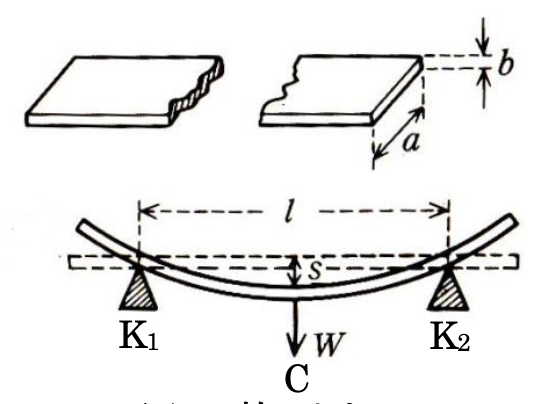
\includegraphics[width=150mm]{actA.png}
  \caption{棒のたわみ}
  \end{center}
\end{figure}

\begin{figure}[h]
  \begin{center}
  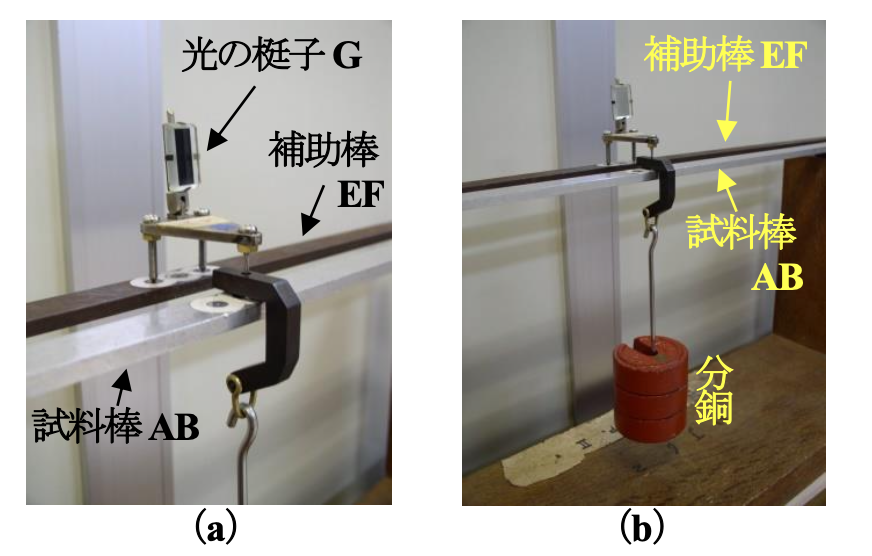
\includegraphics[width=150mm]{actB.png}
  \caption{光の梃子,試料棒,補助棒,分銅の配置図}
  \end{center}
\end{figure}

\begin{figure}[h]
  \begin{center}
  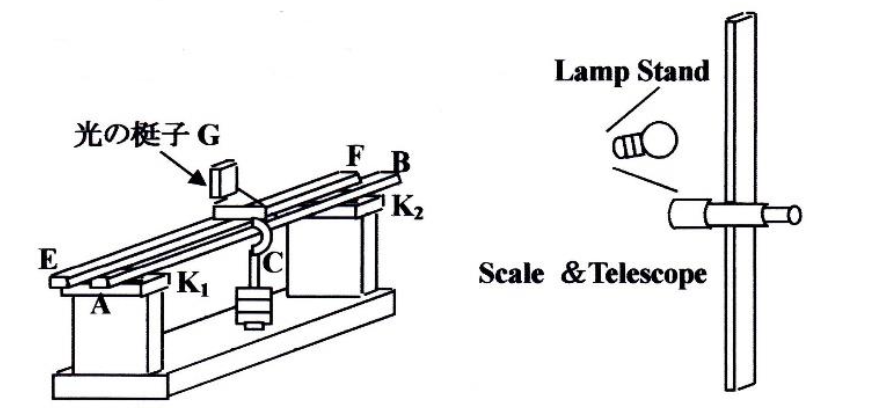
\includegraphics[width=150mm]{actC.png}
  \caption{Ewing の装置配置図}
  \end{center}
\end{figure}

\clearpage


\section{データ処理・結果}




\begin{table}[H]
  \caption{lの測定値}
  \label{table:SpeedOfLight}
  \centering
  \begin{tabular}{|c||r|r|r|r|r|r|r|r|r|r|}
    \hline
    num & l[mm] & r[mm] & $r^2\times10^4[mm^2]$ \\
    \hline\hline
    1 & 402.4 & -0.090 & 81.000 \\
    2 & 402.5 & 0.010 & 1.000 \\
    3 & 402.4 & -0.090 & 81.000 \\
    4 & 402.6 & 0.110 & 121.000 \\
    5 & 402.6 & 0.110 & 121.000 \\
    6 & 402.6 & 0.110 & 121.000 \\
    7 & 402.4 & -0.090 & 81.000 \\
    8 & 402.7 & 0.210 & 441.000 \\
    9 & 402.4 & -0.090 & 81.000 \\
    10 & 402.3 & -0.190 & 361.000 \\
    \hline\hline
    sum & 4024.9 &  & 1490.000 \\
    \hline
    avg & 402.49 &  &  \\

    \hline
  \end{tabular}

\end{table}


  $確率誤差r_lは,理論(1)より,r_l=\pm0.6745\sqrt{\dfrac{1490.000\times10^{-4}}{90}}=\pm0.02744440588[mm].$

\begin{table}[H]
  \caption{Lの測定値}
  \label{table:SpeedOfLight}
  \centering
  \begin{tabular}{|c||r|r|r|r|r|r|r|r|r|r|}
    \hline
    num & L[mm] & r[mm] & $r^2\times10^4[mm^2]$ \\
    \hline\hline
    1 & 30.90 & -0.020 & 4.000 \\
    2 & 30.90 & -0.020 & 4.000 \\
    3 & 30.90 & -0.020 & 4.000 \\
    4 & 30.95 & 0.030 & 9.000 \\
    5 & 30.90 & -0.020 & 4.000 \\
    6 & 30.95 & 0.030 & 9.000 \\
    7 & 30.90 & -0.020 & 4.000 \\
    8 & 30.95 & 0.030 & 9.000 \\
    9 & 30.90 & -0.020 & 4.000 \\
    10 & 30.95 & 0.030 & 9.000 \\
    \hline\hline
    sum & 309.20 &  & 60.000 \\
    \hline
    avg & 30.92 &  &  \\

    \hline
  \end{tabular}


\end{table}

$確率誤差r_Lは,理論(1)より,r_L=\pm0.6745\sqrt{\dfrac{60.000\times10^{-4}}{90}}=\pm0.005507269438[mm].$





\clearpage

\subsection*{鉄}

\begin{table}[H]
  \caption{yの測定値}
  \label{table:SpeedOfLight}
  \centering
  \begin{tabular}{|c||r|r|r|r|r|r|r|r|r|r|}
    \hline
    num & x[g] & y[mm] & $x^2 [mm^2]$ & xy [g*mm] & y' [mm] & v [mm] & $v^2\times10^8 [mm^2]$ \\
    \hline\hline
    1 & 0 & 601.4 & 0 & 0.00 & 601.27 & 0.13 & 1612231.6482 \\
    2 & 200 & 609.2 & 40000 & 121840.00 & 608.64 & 0.56 & 30852595.5396 \\
    3 & 400 & 617.7 & 160000 & 247080.00 & 616.02 & 1.68 & 283561543.3673 \\
    4 & 600 & 624.8 & 360000 & 374880.00 & 623.39 & 1.41 & 199489075.1314 \\
    5 & 800 & 630.3 & 640000 & 504240.00 & 630.76 & -0.46 & 21078799.8544 \\
    6 & 1000 & 638.2 & 1000000 & 638200.00 & 638.13 & 0.07 & 481093.4762 \\
    7 & 1200 & 645.5 & 1440000 & 774600.00 & 645.50 & 0.00 & 467.2749 \\
    8 & 1400 & 653.0 & 1960000 & 914200.00 & 652.87 & 0.13 & 1595567.8670 \\
    9 & 1200 & 645.6 & 1440000 & 774720.00 & 645.50 & 0.10 & 957234.1922 \\
    10 & 1000 & 637.8 & 1000000 & 637800.00 & 638.13 & -0.33 & 10932221.2957 \\
    11 & 800 & 630.2 & 640000 & 504160.00 & 630.76 & -0.56 & 31261130.6815 \\
    12 & 600 & 622.5 & 360000 & 373500.00 & 623.39 & -0.89 & 78782308.2142 \\
    13 & 400 & 615.6 & 160000 & 246240.00 & 616.02 & -0.42 & 17311543.3674 \\
    14 & 200 & 607.9 & 40000 & 121580.00 & 608.64 & -0.74 & 55435302.3066 \\
    15 & 0 & 600.6 & 0 & 0.00 & 601.27 & -0.67 & 45296442.1746 \\

    \hline\hline
    sum & 9800 & 9380.3 & 9240000 & 6233040.00 &  & 0.00 & 778647556.3910 \\

    \hline
  \end{tabular}


\end{table}

理論(5),(6)より,\\

$A=\dfrac{15\times6233040.00-9800\times9380.3}{15\times9240000-9800^2}=0.03685761278$\\

$B=\dfrac{9240000\times9380.3-9800\times6233040.00}{15\times9240000-9800^2}=601.2730263$\\

理論(8)(9)より,\\

$E_A=\pm0.6745\sqrt{\dfrac{15}{15\times9240000-9800^2}\times\dfrac{778647556.3910\times10^{-8}}{13}}=0.00030990$\\

$E_B=\pm0.6745\sqrt{\dfrac{9240000}{15\times9240000-9800^2}\times\dfrac{778647556.3910\times10^{-8}}{13}}=0.24322931$\\

したがって,\\

$A=0.03685761278\pm0.00030990[mm/g]$\\

$B=601.2730263\pm0.24322931[mm]$\\

\begin{figure}[h]
  \begin{center}
  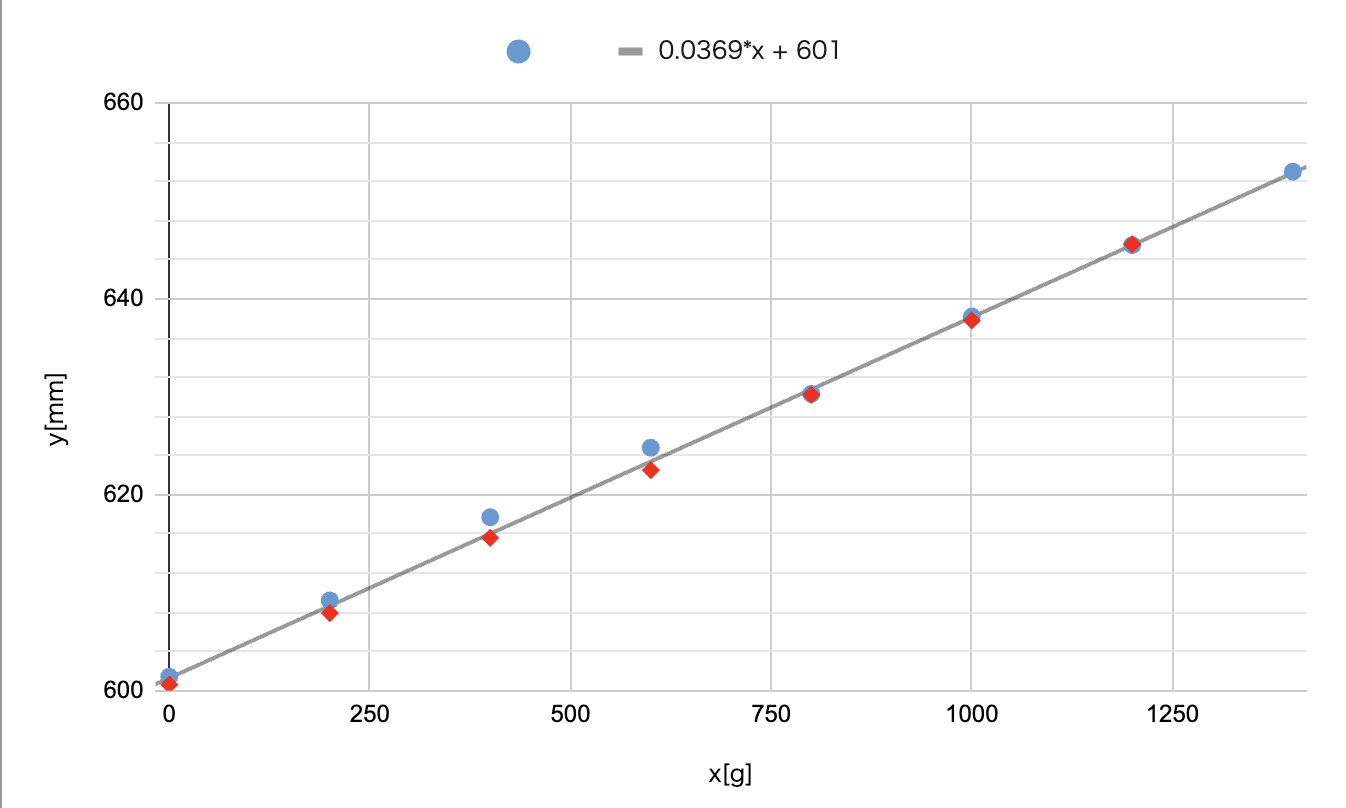
\includegraphics[width=150mm]{actD.png}
  \caption{xとyの関係}
  \end{center}
\end{figure}



\clearpage

\begin{table}[H]
  \caption{aの測定値}
  \label{table:SpeedOfLight}
  \centering
  \begin{tabular}{|c||r|r|r|r|r|r|r|r|r|r|}
    \hline
    num & ゼロ点[mm] & 実測値[mm] & 幅 a[mm] & 残差 r[mm] & $r^2\times10^8[mm^2]$  \\
    \hline\hline
    1 & -0.010 & 15.959 & 15.969 & 0.016 & 27225.000 \\
    2 & 0.000 & 15.945 & 15.945 & -0.008 & 5625.000 \\
    3 & 0.000 & 15.945 & 15.945 & -0.008 & 5625.000 \\
    4 & -0.008 & 15.951 & 15.959 & 0.006 & 4225.000 \\
    5 & 0.000 & 15.956 & 15.956 & 0.003 & 1225.000 \\
    6 & 0.000 & 15.948 & 15.948 & -0.005 & 2025.000 \\
    7 & 0.000 & 15.942 & 15.942 & -0.011 & 11025.000 \\
    8 & -0.003 & 15.947 & 15.950 & -0.003 & 625.000 \\
    9 & 0.000 & 15.971 & 15.971 & 0.018 & 34225.000 \\
    10 & 0.000 & 15.940 & 15.940 & -0.013 & 15625.000 \\
    \hline\hline
    sum &  &  & 159.525 & 0.0000 & 43925.000 \\
    \hline
    avg &  &  & 15.953 &  &  \\

    \hline
  \end{tabular}

\end{table}

$確率誤差r_aは,理論(1)より,r_a=\pm0.6745\sqrt{\dfrac{43925.000\times10^{-8}}{90}}=\pm0.001490104013[mm].$

\begin{table}[H]
  \caption{bの測定値}
  \label{table:SpeedOfLight}
  \centering
  \begin{tabular}{|c||r|r|r|r|r|r|r|r|r|r|}
    \hline
    num & ゼロ点[mm] & 実測値[mm] & 幅 b[mm] & 残差 r[mm] & $r^2\times10^8[mm^2]$  \\
    \hline\hline
    1 & -0.008 & 4.952 & 4.960  & 0.001  & 121.000 \\
    2 & -0.002 & 4.950 & 4.952  & -0.007  & 4761.000 \\
    3 & -0.001 & 4.958 & 4.959  & 0.000  & 1.000 \\
    4 & -0.004 & 4.958 & 4.962  & 0.003  & 961.000 \\
    5 & -0.005 & 4.959 & 4.964  & 0.005  & 2601.000 \\
    6 & 0.000 & 4.960 & 4.960  & 0.001  & 121.000 \\
    7 & -0.002 & 4.959 & 4.961  & 0.002  & 441.000 \\
    8 & 0.000 & 4.957 & 4.957  & -0.002  & 361.000 \\
    9 & -0.005 & 4.956 & 4.961  & 0.002  & 441.000 \\
    10 & 0.000 & 4.953 & 4.953  & -0.006  & 3481.000 \\
    
    \hline\hline
    sum &  &  & 49.589  & 0.0000 & 8445.000 \\
    \hline
    avg &  &  & 4.959 &  &  \\

    \hline
  \end{tabular}

\end{table}

$確率誤差r_bは,理論(1)より,r_b=\pm0.6745\sqrt{\dfrac{8445.000\times10^{-8}}{90}}=\pm0.0006533720109[mm].$

\begin{table}[H]
  \caption{Dの測定値}
  \label{table:SpeedOfLight}
  \centering
  \begin{tabular}{|c||r|r|r|r|r|r|r|r|r|r|}
    \hline
    num & D[mm] & r[mm] & $r^2\times10^4[mm^2]$ \\
    \hline\hline
    1 & 1564.800 & -3.680  & 135424.000 \\
    2 & 1568.10 & -0.380  & 1444.000 \\
    3 & 1569.200 & 0.720  & 5184.000 \\
    4 & 1568.300 & -0.180  & 324.000 \\
    5 & 1568.900 & 0.420  & 1764.000 \\
    6 & 1566.900 & -1.580  & 24964.000 \\
    7 & 1568.800 & 0.320  & 1024.000 \\
    8 & 1569.300 & 0.820  & 6724.000 \\
    9 & 1570.300 & 1.820  & 33124.000 \\
    10 & 1570.200 & 1.720  & 29584.000 \\
    \hline\hline
    sum & 15684.800  & 0.000  & 144140.000 \\
    \hline
    avg  & 1568.480 &  &  \\

    \hline
  \end{tabular}

\end{table}

$確率誤差r_Dは,理論(1)より,r_D=\pm0.6745\sqrt{\dfrac{144140.000\times10^{-4}}{90}}=\pm0.2699311209[mm].$\\

したがって,鉄のYoung率Eは,\\

最確値は$E=\dfrac{1}{2}\dfrac{l^3Dg}{ab^3LA}=\dfrac{1}{2}\times\dfrac{(402.49)^3\times1568.480\times9.79708}{15.953\times(4.959)^3\times30.92\times0.03685761278\times10^{3}}=225953.75[N/mm^2]$\\

確率誤差$r_E^2=(\frac{\partial E}{\partial l}r_{l})^2+(\frac{\partial E}{\partial L}r_{L})^2+(\frac{\partial E}{\partial A}E_{A})^2+(\frac{\partial E}{\partial a}r_{a})^2+(\frac{\partial E}{\partial b}r_{b})^2+(\frac{\partial E}{\partial D}r_{D})^2$\\

$=(\dfrac{3l^2Dg}{2ab^3LA}r_l)^2+(\dfrac{-l^3Dg}{2ab^3AL^2}r_L)^2+(\dfrac{-l^3Dg}{2ab^3LA^2}E_A)^2+(\dfrac{-l^3Dg}{2a^2b^3AL}r_a)^2+(\dfrac{-3l^3Dg}{2ab^4AL}r_b)^2+(\dfrac{l^3g}{2ab^3AL}r_D)^2$\\

$=(\dfrac{3\times(402.49)^2\times1568.48\times9.79708}{2\times15.953\times(4.959)^3\times30.92\times0.03685761278\blue{\times10^3}}\times0.02744440588)^2$\\

$+(\dfrac{-(402.49)^3\times1568.48\times9.79708}{2\times15.953\times(4.959)^3\times0.03685761278\times(30.92)^2\blue{\times10^3}}\times0.005507269438)^2$\\

$+(\dfrac{-(402.49)^3\times1568.48\times9.79708}{2\times15.953\times(4.959)^3\times30.92\times(0.03685761278)^2\blue{\times10^3}}\times0.00030990)^2$\\

$+(\dfrac{-(402.49)^3\times1568.48\times9.79708}{2\times(15.953)^2\times(4.959)^3\times0.03685761278\times30.92\blue{\times10^3}}\times0.001490104013)^2$\\

$+(\dfrac{-3\times(402.49)^3\times1568.48\times9.79708}{2\times(15.953)^2\times(4.959)^4\times0.03685761278\times30.92\blue{\times10^3}}\times0.0006533720109)^2$\\

$+(\dfrac{(402.49)^3\times9.79708}{2\times15.953\times(4.959)^3\times30.92\times0.03685761278\blue{\times10^3}}\times0.2699311209)^2$\\

$\blue{=(40.24541302)^2+(46.22102191)^2+(1899.826419)^2+(21.1054088)^2+(89.31146684)^2+(38.88602243)^2}$\\



=$3623030.597[N^2/mm^4$]\\

$したがって,r_E=\pm1903.426016[N/mm^2].$\\

よって,$E=225953.75\pm1903.426016=(2.26\pm0.02)\times10^5[N/mm^2].$





\clearpage

\subsection*{真鍮}

\begin{table}[H]
  \caption{yの測定値}
  \label{table:SpeedOfLight}
  \centering
  \begin{tabular}{|c||r|r|r|r|r|r|r|r|r|r|}
    \hline
    num & x[g] & y[mm] & $x^2 [mm^2]$ & xy [g*mm] & y' [mm] & v [mm] & $v^2\times10^8 [mm^2]$ \\
    \hline\hline
    1 & 0 & 365.6 & 0 & 0.00 & 364.78 & 0.82 & 67737231.6482 \\
    2 & 200 & 380.7 & 40000 & 76140.00 & 380.87 & -0.17 & 2881059.5568 \\
    3 & 400 & 396.8 & 160000 & 158720.00 & 396.96 & -0.16 & 2640625.0000 \\
    4 & 600 & 413.2 & 360000 & 247920.00 & 413.06 & 0.14 & 2094875.3463 \\
    5 & 800 & 429.4 & 640000 & 343520.00 & 429.15 & 0.25 & 6349073.7535 \\
    6 & 1000 & 445.7 & 1000000 & 445700.00 & 445.24 & 0.46 & 21087430.7479 \\
    7 & 1200 & 460.9 & 1440000 & 553080.00 & 461.33 & -0.43 & 18796788.4349 \\
    8 & 1400 & 477.8 & 1960000 & 668920.00 & 477.43 & 0.37 & 13963988.9197 \\
    9 & 1200 & 461.8 & 1440000 & 554160.00 & 461.33 & 0.47 & 21757314.7507 \\
    10 & 1000 & 444.8 & 1000000 & 444800.00 & 445.24 & -0.44 & 19429536.0111 \\
    11 & 800 & 428.8 & 640000 & 343040.00 & 429.15 & -0.35 & 12112231.6482 \\
    12 & 600 & 412.6 & 360000 & 247560.00 & 413.06 & -0.46 & 20726454.2936 \\
    13 & 400 & 396.5 & 160000 & 158600.00 & 396.96 & -0.46 & 21390625.0000 \\
    14 & 200 & 380.7 & 40000 & 76140.00 & 380.87 & -0.17 & 2881059.5568 \\
    15 & 0 & 364.9 & 0 & 0.00 & 364.78 & 0.12 & 1513547.4377 \\

    \hline\hline
    sum & 9800 & 6260.2 & 9240000 & 4318300.00 &  & 0.00 & 235361842.1053 \\

    \hline
  \end{tabular}

\end{table}

理論(5),(6)より,\\

$A=\dfrac{15\times4318300.00-9800\times6260.2}{15\times9240000-9800^2}=0.08046381579$\\

$B=\dfrac{9240000\times6260.2-9800\times4318300.00}{15\times9240000-9800^2}=364.7769737$\\

理論(8)(9)より,\\

$E_A=\pm0.6745\sqrt{\dfrac{15}{15\times9240000-9800^2}\times\dfrac{235361842.1053\times10^{-8}}{13}}=0.00017038$\\

$E_B=\pm0.6745\sqrt{\dfrac{9240000}{15\times9240000-9800^2}\times\dfrac{235361842.1053\times10^{-8}}{13}}=0.13372527$\\

したがって,\\

$A=0.08046381579\pm0.00017038[mm/g]$\\

$B=364.7769737\pm0.13372527[mm]$\\

\begin{figure}[h]
  \begin{center}
  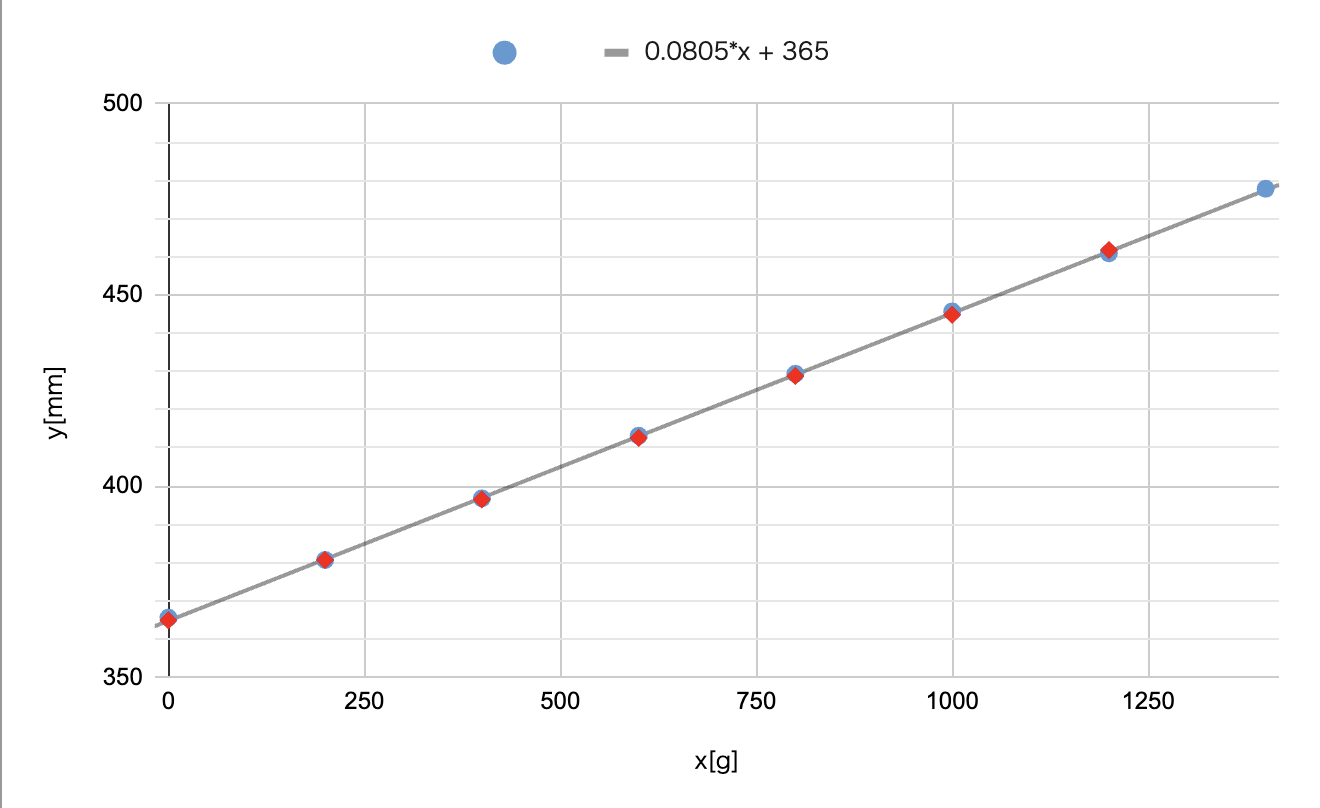
\includegraphics[width=150mm]{actE.png}
  \caption{xとyの関係}
  \end{center}
\end{figure}


\clearpage

\begin{table}[H]
  \caption{aの測定値}
  \label{table:SpeedOfLight}
  \centering
  \begin{tabular}{|c||r|r|r|r|r|r|r|r|r|r|}
    \hline
    num & ゼロ点[mm] & 実測値[mm] & 幅 a[mm] & 残差 r[mm] & $r^2\times10^8[mm^2]$  \\
    \hline\hline
    1 & -0.008 & 15.982 & 15.990 & 0.005 & 2401.000 \\
    2 & -0.008 & 15.979 & 15.987 & 0.002 & 361.000 \\
    3 & -0.012 & 15.979 & 15.991 & 0.006 & 3481.000 \\
    4 & -0.009 & 15.985 & 15.994 & 0.009 & 7921.000 \\
    5 & -0.001 & 15.981 & 15.982 & -0.003 & 961.000 \\
    6 & -0.004 & 15.979 & 15.983 & -0.002 & 441.000 \\
    7 & -0.002 & 15.982 & 15.984 & -0.001 & 121.000 \\
    8 & -0.001 & 15.979 & 15.980 & -0.005 & 2601.000 \\
    9 & -0.002 & 15.978 & 15.980 & -0.005 & 2601.000 \\
    10 & -0.001 & 15.979 & 15.980 & -0.005 & 2601.000 \\
    
    \hline\hline
    sum &  &  & 159.851 & 0.0000 & 15125.000 \\
    \hline
    avg &  &  & 15.985 &  &  \\

    \hline
  \end{tabular}

\end{table}

$確率誤差r_aは,理論(1)より,r_a=\pm0.6745\sqrt{\dfrac{15125.000\times10^{-8}}{90}}=\pm0.0008743964605[mm].$

\begin{table}[H]
  \caption{bの測定値}
  \label{table:SpeedOfLight}
  \centering
  \begin{tabular}{|c||r|r|r|r|r|r|r|r|r|r|}
    \hline
    num & ゼロ点[mm] & 実測値[mm] & 幅 b[mm] & 残差 r[mm] & $r^2\times10^8[mm^2]$  \\
    \hline\hline
    1 & -0.004 & 5.008 & 5.012  & 0.000  & 4.000 \\
    2 & -0.009 & 5.002 & 5.011  & -0.001  & 144.000 \\
    3 & -0.010 & 5.003 & 5.013  & 0.001  & 64.000 \\
    4 & -0.011 & 5.007 & 5.018  & 0.006  & 3364.000 \\
    5 & -0.008 & 5.000 & 5.008  & -0.004  & 1764.000 \\
    6 & -0.008 & 5.006 & 5.014  & 0.002  & 324.000 \\
    7 & -0.009 & 5.005 & 5.014  & 0.002  & 324.000 \\
    8 & -0.006 & 5.009 & 5.015  & 0.003  & 784.000 \\
    9 & -0.009 & 5.002 & 5.011  & -0.001  & 144.000 \\
    10 & -0.005 & 5.001 & 5.006  & -0.006  & 3844.000 \\
    
    \hline\hline
    sum &  &  & 50.122  & 0.0000 & 10760.000 \\
    \hline
    avg &  &  & 5.012 &  &  \\

    \hline
  \end{tabular}

\end{table}

$確率誤差r_bは,理論(1)より,r_b=\pm0.6745\sqrt{\dfrac{10760.000\times10^{-8}}{90}}=\pm0.0007375081687[mm].$



\begin{table}[H]
  \caption{Dの測定値}
  \label{table:SpeedOfLight}
  \centering
  \begin{tabular}{|c||r|r|r|r|r|r|r|r|r|r|}
    \hline
    num & D[mm] & r[mm] & $r^2\times10^2[mm^2]$ \\
    \hline\hline
    1 & 1564.200 & 10.486  & 10995.61960 \\
    2 & 1564.50 & 10.786  & 11633.77960 \\
    3 & 1550.800 & -2.914  & 849.13960 \\
    4 & 1549.100 & -4.614  & 2128.89960 \\
    5 & 1549.000 & -4.714  & 2222.17960 \\
    6 & 1552.200 & -1.514  & 229.21960 \\
    7 & 1550.100 & -3.614  & 1306.09960 \\
    8 & 1553.100 & -0.614  & 37.69960 \\
    9 & 1555.140 & 1.426  & 203.34760 \\
    10 & 1549.000 & -4.714  & 2222.17960 \\
    \hline\hline
    sum & 15537.140  & 0.000  & 27829.61800 \\
    \hline
    avg  & 1553.714 &  &  \\

    \hline
  \end{tabular}

\end{table}

$確率誤差r_Dは,理論(1)より,r_D=\pm0.6745\sqrt{\dfrac{27829.61800\times10^{-2}}{90}}=\pm1.186080926[mm].$\\

したがって,真鍮のYoung率Eは,\\

最確値は$E=\dfrac{1}{2}\dfrac{l^3Dg}{ab^3LA}=\dfrac{1}{2}\times\dfrac{(402.49)^3\times1553.714\times9.79708}{15.985\times(5.012)^3\times30.92\times0.08046381579\times10^{3}}=99139.45[N/mm^2]$\\

確率誤差$r_E^2=(\frac{\partial E}{\partial l}r_{l})^2+(\frac{\partial E}{\partial L}r_{L})^2+(\frac{\partial E}{\partial A}E_{A})^2+(\frac{\partial E}{\partial a}r_{a})^2+(\frac{\partial E}{\partial b}r_{b})^2+(\frac{\partial E}{\partial D}r_{D})^2$\\

$=(\dfrac{3l^2Dg}{2ab^3LA}r_l)^2+(\dfrac{-l^3Dg}{2ab^3AL^2}r_L)^2+(\dfrac{-l^3Dg}{2ab^3LA^2}E_A)^2+(\dfrac{-l^3Dg}{2a^2b^3AL}r_a)^2+(\dfrac{-3l^3Dg}{2ab^4AL}r_b)^2+(\dfrac{l^3g}{2ab^3AL}r_D)^2$\\

$=(\dfrac{3\times(402.49)^2\times1553.714\times9.79708}{2\times15.985\times(5.012)^3\times30.92\times0.08046381579\blue{\times10^3}}\times0.02744440588)^2$\\

$+(\dfrac{-(402.49)^3\times1553.714\times9.79708}{2\times15.985\times(5.012)^3\times0.08046381579\times(30.92)^2\blue{\times10^3}}\times0.005507269438)^2$\\

$+(\dfrac{-(402.49)^3\times1553.714\times9.79708}{2\times15.985\times(5.012)^3\times30.92\times(0.08046381579)^2\blue{\times10^3}}\times0.00017038)^2$\\

$+(\dfrac{-(402.49)^3\times1553.714\times9.79708}{2\times(15.985)^2\times(5.012)^3\times0.08046381579\times30.92\blue{\times10^3}}\times0.0008743964605)^2$\\

$+(\dfrac{-3\times(402.49)^3\times1553.714\times9.79708}{2\times(15.985)^2\times(5.012)^4\times0.08046381579\times30.92\blue{\times10^3}}\times0.0007375081687)^2$\\

$+(\dfrac{(402.49)^3\times9.79708}{2\times15.985\times(5.012)^3\times30.92\times0.08046381579\blue{\times10^3}}\times1.186080926)^2$\\

$\blue{=(17.65281314)^2+(20.27388966)^2+(209.8626124)^2+(5.421417274)^2+(43.75161736)^2+(75.6589531)^2}$\\

=$52432.84147[N^2/mm^4$]\\

$したがって,r_E=\pm228.9821859[N/mm^2].$\\

よって,$E=99139.45\pm228.9821859=(9.91\pm0.02)\times10^4[N/mm^2].$



 
 
\section{考察}

 $鉄,真鍮のYoung率の公称値はそれぞれ,1.9\times10^5〜2.1\times10^5[mm],9.7\times10^4〜1.02\times10^5[mm]である.真鍮は実験値と公称値が一致したが,鉄は確率誤差の範囲内でも一致しない,大きい値となった(誤差は+6.66〜8.57\%).鉄のYoung率の実験値が大きくなってしまった理由として以下の2つが考えられる.$\\

 \begin{enumerate}
 \item 実験手法によるもの
 \item 加工硬化によるもの
\end{enumerate}

1.で考えられるのは,分銅をかける位置が鉄棒の重心からズレていた,若しくは分銅を増やすごとに,分銅の位置がズレてしまい,力の作用点が変わっていた可能性がある.たとえ同じ試料でも厚みは均一でないため,これらの人為的ミスが結果に影響していることは大いにあり得る.(特に最小二乗法の計算において鉄は真鍮に比べ,各データと近似直線との誤差が大きかった)\\

2.は可能性は低いが,Young率が公称値より「大きい」という実験結果をふまえ考察に含めた.

\end{document}
